\documentclass{article}
\usepackage[utf8]{inputenc}
\usepackage{float}
\usepackage{graphicx}
\title{Manual: wxMaxima}
\begin{document}
\maketitle
\tableofcontents
\section{¿Qué es \textit{Maxima}?}
\textit{Maxima} es de los más antiguos CAS's (Computer Algebra Systems). Fué creado por el MIT en la década de 1960 inicialmente Macsyma (project MAC's SYmbolic MAnipulator). Diseñado para ser utilizado en varias instituciones en la época. En 1980 verciones derivadas tomaron el nombre de \textit{Maxima}, hoy en día se distribuye como un software libre.
\section{Objetivo}
El siguiente manual tiene como objetivo ayudar al usuario del sistema \textbf{Maxima}. Dentro de éste se proporcionarán tanto comandos como ejemplos para mostrar al lector cómo hacer uso del programa.
\section{La Interfaz Gráfica}
La interfaz utilizada en wxMaxima permite al usuario introducir de una manera sencilla lo que desea calcular. Existen distintos tipos de opincludegraphicseraciones realizables en wxMaxima. Algunas de ellas son: aritmética, solución de ecuaciones, graficar funciones, resolver límites, derivar e integrar.
\subsection{Aritmética}
Algo a tomar en cuenta es que al ingresar valores p. ej. dos sumandos. Éstos son asociados como valores de entrada, mientras que su resultado como valor de salida. Los valores de entrada van denotados por un símbolo de porcentaje, la letra \textit{i} (proveniente de la palabra en inglés input) y un número (éste depende del orden asignado a los valores de entrada). Siendo por ejemplo \%i1 el "nombre" asignado al primer valor o valores de entrada introducidos. En el caso de ser valor de salida solo se cambia la letra \textit{i} por la \textit{o}.\\

	\begin{figure}[H]
		\centering
        \includegraphics[width=\linewidth]{arit.png}
	\end{figure} 
 
\subsection{Solución de Ecuaciones}
La herramienta de solución de ecuaciones es muy importante. Para hacer uso de ella necesitamos introducir el comando \textit{solve} después se abre un paréntesis, en éste irán dos cosas, la ecuación a resolver con sus variables dentro de corchetes además separado por una coma y también entre corchetes las variables en la ecuación.

	\begin{figure}[H]
		\centering
        \includegraphics[width=\linewidth]{ecu.png}
	\end{figure}
    
\subsection{Graficar Funciones}
Al momento de graficar funciones utilizamos el comando contour. Ejemplos de éste caso son los siguientes:

	\begin{figure}[H]
		\centering
        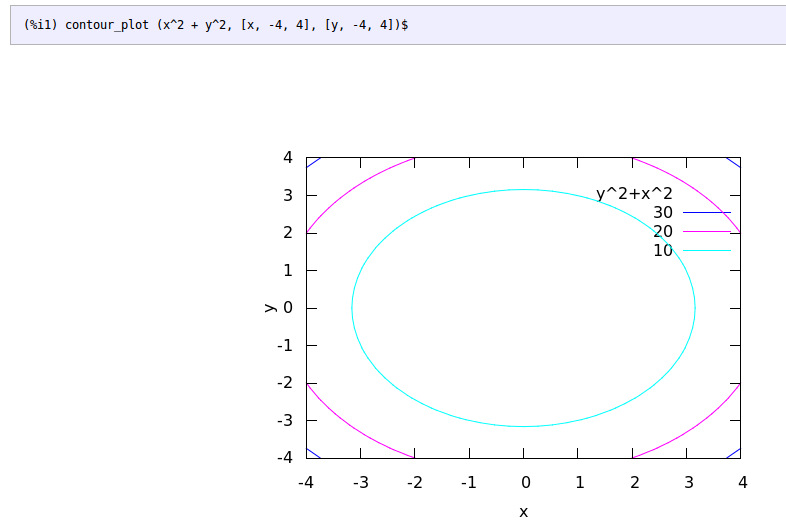
\includegraphics[width=\linewidth]{grax.png}
	\end{figure}
    
    \begin{figure}[H]
    	\centering
        \includegraphics[width=\linewidth]{gr2.png}
    \end{figure}
    
\section{Referencias}

	\begin{itemize}
		\item \textnormal{http://maxima-online.org/}
    	\item \textnormal{http://www.scotchildress.com/wxmaxima/}
        \item \textnormal{http://web.csulb.edu/~woollett/}
	\end{itemize}

\end{document}
